\documentclass[a4paper]{ltjsarticle}

\usepackage{amsmath} % 数式を記述するためのパッケージ
\usepackage{graphicx} % 画像を挿入するためのパッケージ
\usepackage{url} % URLを記述するためのパッケージ
\usepackage{here} % 図表をその場所に表示するためのパッケージ
\usepackage{luacode} % ソースコードを記述するためのパッケージ
\usepackage{titling} % タイトルをカスタマイズするためのパッケージ
\usepackage{fancyhdr} % ヘッダーをカスタマイズするためのパッケージ
\usepackage{siunitx}
\usepackage{multirow}
\usepackage{bigdelim}
\usepackage{amssymb}
\usepackage{listings}
\usepackage{xcolor}
\usepackage{multicol}
\usepackage[subrefformat=parens]{subcaption}

\definecolor{codegreen}{rgb}{0,0.6,0}
\definecolor{codegray}{rgb}{0.5,0.5,0.5}
\definecolor{codepurple}{rgb}{0.58,0,0.82}
\definecolor{backcolour}{rgb}{0.95,0.95,0.92}

\lstdefinestyle{mystyle}{
    backgroundcolor=\color{backcolour},   
    commentstyle=\color{codegreen},
    keywordstyle=\color{blue},
    numberstyle=\tiny\color{codegray},
    stringstyle=\color{codepurple},
    basicstyle=\ttfamily\footnotesize,
    breakatwhitespace=false,         
    breaklines=true,                 
    captionpos=b,                    
    keepspaces=true,                 
    numbers=left,                    
    numbersep=5pt,                  
    showspaces=false,                
    showstringspaces=false,
    showtabs=false,                  
    tabsize=2,
    title=\lstname
}
\lstset{style=mystyle}


\preauthor{\begin{flushright}} % authorを右寄せにする
\postauthor{\end{flushright}}
\predate{\begin{flushright}} % dateを右寄せにする
\postdate{\end{flushright}}

\pagestyle{fancy}
\lhead{電気電子情報実験・演習第一 E1実験レポート}
\rhead{03240403 井上聡士}
\cfoot{\thepage}
\renewcommand{\headrulewidth}{0pt}


\title{電気電子情報実験・演習第一 E1実験レポート}
\author{電子情報工学科 \\ 03240403 井上聡士}
\date{2024年6月22日}


\begin{document}
\maketitle % タイトルページを表示する
\section{平等電界の火花電圧}
\subsection{右側領域におけるパッシェン曲線の測定}
距離を$d = 1, 3, 5\,\si{\milli\meter}$、圧力を$p=1000, 3000, 10000, 30000, 50000\,\si{\pascal}$に調整し、計15種類の条件において、各3回ずつ放電した際の電圧を記録した。
距離はマイクロメーターを使用し調整した。
球の間の抵抗を測定しながら、距離を徐々に縮めたときに抵抗値が有限となるときの値を零点とした結果、最初に測った際は$\SI{6.75}{\milli\meter}$であった。
圧力の測定はすべて有効数字1桁でデジタルで数値が表示されるピラニー真空計を使用し、比較的大きな圧力を計測するのに使用するブルドン管式真空計は使用しなかった。

\subsection{左側領域におけるパッシェン曲線の測定}
気圧を$p=\SI{1000}{\pascal}$程度で固定し、距離を$d=0.1, 0.2, 0.3, 0.5, 0.7, 1.0\,\si{\milli\meter}$、およびマイクロメーターが最小値(0)となる位置での火花電圧を、各3回ずつ測定した。
この時もピラニー真空計のみを使用し気圧を測定した。
また、再びマイクロメーターの零点を測定しなおしたところ、目盛りは$\SI{6.32}{\milli\meter}$であった。

\subsection{結果} \label{sec:equal_result}
\begin{figure}[htbp]
    \centering
    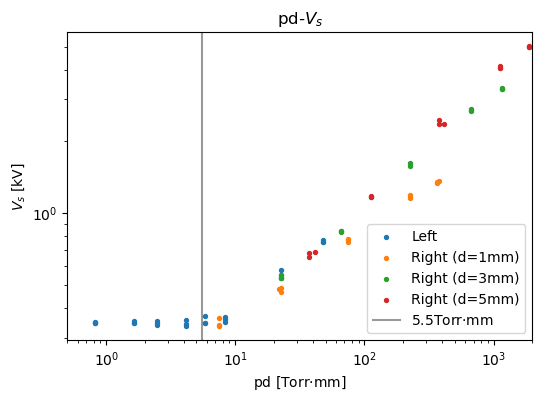
\includegraphics[width=0.7\linewidth]{./images/equal_measured.png}
    \caption{平等電界の火花電圧の測定値}
    \label{fig:equal_measured}
\end{figure}
図\ref{fig:equal_measured}に、平等電界の火花電圧の測定値を示す。
縦軸は火花電圧$V_S$、横軸は圧力と距離の積$pd\,[\text{Torr\cdot mm}]$である。
$760\,\text{Torr} = \SI{1013.25}{\hecto\pascal}$であり、$1\,\text{Torr} = \SI{133.32}{\pascal}$である。

右側領域のパッシェン曲線について、距離が大きい$d=3, 5\,\si{\milli\meter}$については、ほぼ同じ曲線上に乗っていると考えられるが、$d=\SI{1}{\milli\meter}$の曲線がほかの2曲線から大きく外れている。

左側領域のパッシェン曲線については、$10\text{Torr}\cdot\si{\milli\meter}$程度までは、距離に関係なく電圧$V_S$がほぼ一定であり、その電圧は$\SI{0.35}{\kilo\volt}$程度であった。

\subsection{平等電界の理論値の導出}
電圧が十分大きく、\gamma 作用が存在するとき、全電流$I$は、$I_0$を陰極での電子電流、$d$を電極間隔、$\alpha$を衝突電離係数、$\gamma$を1個の正イオンが放出させることの出来る電子の数とすると、以下のように表される。
\begin{equation}
    I = I_0\frac{\exp(\alpha d)}{1-\gamma\left(\exp(\alpha d)-1\right)}
\end{equation}
このとき、上式の分母が0になると、電流は無限大になり、電流は継続することになる(Townsendの火花条件)。
\begin{equation}
    \alpha d = \log(1+\frac{1}{\gamma}) \label{eq:townsend}
\end{equation}
また、衝突電離係数$\alpha$は、$A, B$を定数、$p$を気圧、$E$を電界強度として($E = V_S/d$)、以下のように表されることが経験則的に知られている。
\begin{equation}
    \frac{\alpha}{p} = A\exp(-\frac{Bp}{E}) \label{eq:alpha}
\end{equation}
これを解くと、$V_S$は以下の式で表される。
\begin{equation}
    V_S = \frac{Bpd}{\log(pd) + \log\left(\frac{A}{\log\left(1+1/\gamma\right)}\right)}
\end{equation}
以降、便宜上$A' = \frac{A}{\log(1+1/\gamma)}$とする。
このとき、最小値を取る$pd$は、$\frac{dV_S}{d(pd)} = 0$を満たし、これを解くと、
\begin{equation}
    (pd)_{\text{min}} = \frac{e}{A'}
\end{equation}
で最小値
\begin{equation}
    V_{S\text{min}} = \frac{Be}{A'}
\end{equation}
を取る。

大気中の放電の文献値は、$A'=\SI{0.38}{Torr^{-1}.mm^{-1}}$、$B=\SI{36}{V.Torr^{-1}.mm^{-1}}$である\cite{Report 1}。
ただし、文献により値が大きく異なり、$A'=0.29\sim0.48\,\si{Torr^{-1}.mm^{-1}}$、$B=36.5\sim64.9\,\si{V.Torr^{-1}.mm^{-1}}$などの文献値が存在する\cite{Report 2}。
$\gamma$については、明確に記している文献は見つからなかったが、0.01\sim0.1程度であるとする文献が多かった\cite{Journal 1}。

\subsection{PC演習・シューマンの条件式に基づく火花電圧の予測}
与えられた$V=\SI{1}{kV}$の時の電界の強度$E$をもとに、電気力線に沿って電離係数$\alpha$を経路積分した。
ただし、$\alpha$は教科書にあるように、電界$E\si{V.cm^{-1}}$、気圧$p\si{Torr}$から次の式で与えられた。
\begin{equation}
    \alpha(E) = \begin{cases}
        0 & (E/p < 31.6) \\
        \frac{p}{10000}\cdot(1.047(E/p-28.5)^2 - 12.6) & (31.6 \leq E/p < 60.0) \\
        (1 - 0.00674755(E/p-60))\cdot\frac{p}{10000}\cdot(1.047(E/p-28.5)^2 - 12.6) & (60.0 \leq E/p < 100.0) \\
        15.0\cdot p\exp\left(\frac{-365}{E/p}\right) & (100.0 \leq E/p)
    \end{cases} \label{eq:alpha_sim}
\end{equation}
このとき、最大13本与えられた電気力線のうち、いずれかの電気力線に沿った線積分$\int\alpha dx$が閾値$K=10$を超えるとき、その電気力線に沿った経路で放電が起こると仮定した。
これを求めるために、$V_S$による二分探索を使用し、放電開始の電圧$V_S$を求めた。
\begin{multicols}{2}
    \begin{lstlisting}[language=python, title={二分探索による$V_S$の検証}]
    def has_spark(data_gap: pd.DataFrame, V, p):
        return any(get_K_line(line, V, p)*2 >= K for line_index, line in data_gap.groupby("No."))
        return any(K_calc >= K for K_calc in get_K(data_gap, V, p))
    
    # V in kV, p in Torr, E in V/cm
    def get_K(data_gap: pd.DataFrame, V, p):
        return [2*get_K_line(line, V, p) for line_index, line in data_gap.groupby("No.")]
    
    def get_K_line(data_line: pd.DataFrame, V, p):
        arr_alpha = valpha(data_line["|E| [kV/cm]"]*V*1000, p)
        return linear_calculus(data_line[["r[cm]", "z[cm]"]].to_numpy(), arr_alpha)
        
    def linear_calculus(coords, values):
        assert len(coords) == len(values)
        sum = 0
        for i in range(len(coords)-1):
            sum += np.sqrt((coords[i+1][0]-coords[i][0])**2+(coords[i+1][1]-coords[i][1])**2) * (values[i]+values[i+1])/2
        return sum
    
    def alpha(E, p):
        Edp = E/p
        if Edp < 31.6:
            return 0
        elif Edp < 60.0:
            return p/10000*(1.047*(Edp-28.5)**2-12.6)
        elif Edp < 100.0:
            return (1-0.00674755*(Edp-60))*p/10000*(1.047*(Edp-28.5)**2-12.6)
        else:
            return 15.0*p*np.exp(-365/Edp)
    valpha = np.vectorize(alpha, excluded=["p"])
    
    def binary_search(Vmin, Vmax, data_gap, p):
        V_pivot = (Vmin+Vmax)/2
        if Vmax-Vmin < 0.005:
            return V_pivot
        is_spark_pivot = has_spark(data_gap, V_pivot, p)
        if (is_spark_pivot):
            return binary_search(Vmin, V_pivot, data_gap, p)
        else:
            return binary_search(V_pivot, Vmax, data_gap, p)
    \end{lstlisting}
\end{multicols}
\begin{figure}
    \centering
    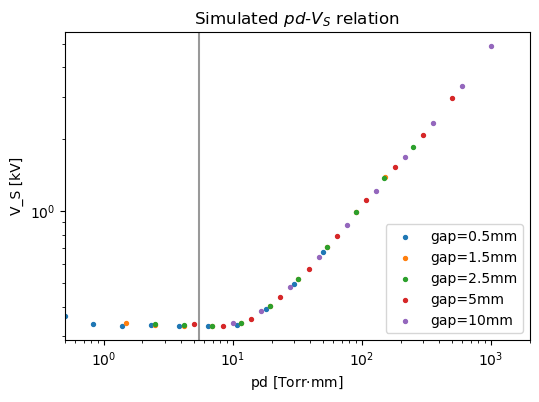
\includegraphics[width=0.7\linewidth]{./images/equal_simulated.png}
    \caption{シューマンの条件式に基づくシミュレーション結果}
    \label{fig:equal_simulated}
\end{figure}
図\ref{fig:equal_simulated}に、シミュレーション結果を示す。
ギャップ長$d$によりわずかにばらつきはあるものの、どの値も基本的に一直線上に乗ることがわかる。
また、pdが小さい領域においては、$V_S$がほぼ一定になることもわかる。

\subsection{考察}
\begin{figure}[htbp]
    \centering
    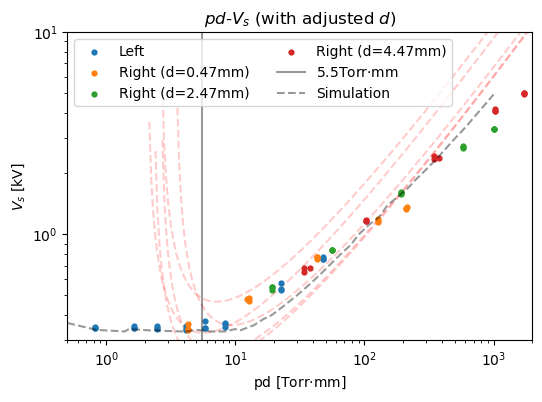
\includegraphics[width=0.7\linewidth]{./images/equal_all.png}
    \caption{平等電界の火花電圧の実測値、理論値、シミュレーションの比較}
    \label{fig:equal_all}
\end{figure}
まず、\ref{sec:equal_result}節で述べたように、$d$によるばらつきを考える。
$d$が小さいときにばらつきの影響が大きく、ほかの曲線から外れる原因として最も考えられるのは、零点の誤差である。
零点でのマイクロメーターの目盛りを$x_0$、計測時の目盛りを$x$とすると、$d=x_0-x$で表されるが、$x_0$の誤りが大きいと$d$にも誤りが生じる。
特に、この誤りは相対的に$d$が小さいときに顕著であり、さらに対数グラフであることにより、ばらつきが大きく見える(例えば、$\SI{1}{mm}$に対する$\SI{0.2}{mm}$の誤差は$\SI{5}{mm}$に対してより相対的に大きい)。
特に、$d=\SI{1}{mm}$の曲線は他の曲線より傾きが小さいが、これは計算した$d$が実際の$d$より大きい、すなわち$x_0$が実際より大きいと考えられる。
実際、最初に零点を計測した際は$\SI{6.75}{mm}$であり、この値を使用し$pd$を求めたが、2回目に測定しなおした際の零点は$\SI{6.32}{mm}$であった。
$d_0$として$\SI{6.32}{mm}$を使用すると、$d=\SI{1}{mm}$の曲線は他の曲線に近づいた(図\ref{fig:equal_all})。

図\ref{fig:equal_all}に、平等電界の火花電圧の$d_0$を補正した実測値、理論値、シミュレーションの比較を示す。
実測値とシミュレーション値は、$pd$の小さい領域を含めてよく一致していた。
しかし、理論値とは一致せず、$pd$が大きい部分ではある程度一致しているように見えたが、$pd$の小さい部分では大きくずれており、理論値と違って$V_S$がほぼ一定であった。
これは、距離が離れたところから出ている電気力線が関係あるかと思われる。
そもそも式\ref{eq:alpha}は、式\ref{eq:alpha_sim}の式の$E/p\geq100.0$で成立する式と似ており、文献値にはかなりのばらつきもあることから、十分大きな範囲で成立する$\alpha$の近似であると考えられる。
式\ref{eq:alpha_sim}の数値15.0、365を単位換算すると$A=\SI{1.5}{Torr^{-1}.mm^{-1}}$、$B=\SI{36.5}{V.Torr^{-1}.mm^{-1}}$となるが、これは文献値と似ており、$\gamma=10^{-2}\sim10^{-1}$程度と考えると$A'$の値も合致する。
また、式\ref{eq:townsend}の式も、一様な電界$\alpha$を距離$d$に沿って積分したものと考えることもでき、$log(1+1/\gamma)$も$K$と捉えられる。
したがって、この理論値の導出はシミュレーションと同様のことをしている。

しかし、この理論値の導出は、あくまで一様な電界に対してのものであり、このような近似が成立するのは、平板コンデンサなどの電場が一意になる場合か、球の$r=0$付近の電気力線(No.1)に沿った場合である。
しかし、実際の球電極では、与えられたデータシートにあるように、より遠くから出ている電気力線が存在する。
これらの電気力線に沿った$\alpha$の経路積分がNo.1より大きくなる場合、No.1付近では放電の起きない電圧でも他の場所で放電が起こる可能性がある。
したがって、理論値で求めた$V_S$よりも低い$V_S$でも放電が起きうるのである。

また、不正確な近似ではあるが、理論値$V_{S\text{theory}}$が極小となる$d$の値$d_{\text{min}}$より左の領域($d'<d_{\text{min}}$)では、球電極の表面を考えると$d_{min}$を含む$d'$以上の全ての$d$において放電が起こる可能性があるため、極小である$d_{\text{min}}$での値$V_{S\text{min}}$でも放電は可能で、結果的に$V_S(d) = V_{S\text{min}}$となる、と解釈できる。
これにより、理論値からの大幅な乖離と、$V_S$が$pd$が小さいときほぼ一定であることが説明できる。

\section{グロー放電の観察}
$50\sim5000\,\si{pa}$の計6点について、グロー放電の観察を行った。
グロー放電の開始する電流$I$から徐々に$I$を大きくし、観測された電圧$V$に$R=\SI{5.26}{\mega\ohm}$に流れる電流分の補正をかけた。
グロー放電が開始する直前の電流では、火花放電のように不規則に電流が流れる現象が観察された。
グロー放電が開始すると、電流は安定し、紫色の光が極間で観測された。
さらに電流を大きくすると、陰極と陽極で別れ、異なる色の光を放射することもあった。
これは、スペクトルの観測の実験でも同様だが、陰極の電圧と陽極の電圧の状況が大きく異なることによる。
陰極側は電圧が急激に変化し、陽極側は緩やかに変化することが知られている。

\begin{figure}
    \centering
    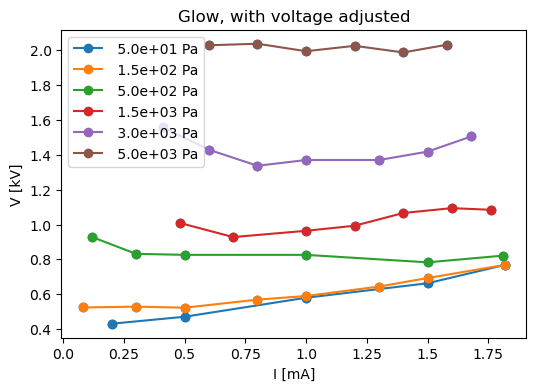
\includegraphics[width=0.7\linewidth]{./images/glow.png}
    \caption{グロー放電の電流-電圧特性}
    \label{fig:glow}
\end{figure}
図\ref{fig:glow}に、グロー放電の電流-電圧特性を示す。
図のように、電流にほぼ寄らず電圧が一定であることが分かった。
前期グローや異常グローなどの電圧変動が観測されなかったのは、測定した電流の領域のためと考えられる。

\section{不平等電界の火花電圧}
円錐-平板電極の火花電圧を測定した。
ただし、時間の都合上本来計測するべき$d$の一部は計測できなかった。
\begin{figure}
    \centering
    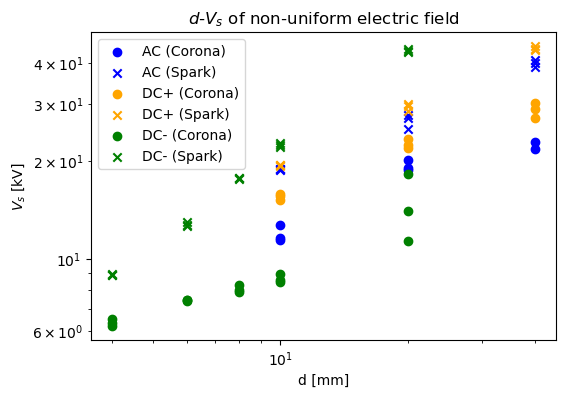
\includegraphics[width=0.7\linewidth]{./images/unequal.png}
    \caption{不平等電界の火花電圧の測定値}
    \label{fig:unequal}
\end{figure}
図\ref{fig:unequal}に、不平等電界のコロナ放電の電圧と火花電圧の測定値を示す。
印加電圧の種類によりコロナ放電電圧・火花電圧ともに値が大きく変わる。
これは極性効果と呼ばれるもので、円錐が陰極の時に火花電圧は小さく、陽極の時にもっとも大きかった。
これは、円錐が陰極の場合、電場も大きく電子雪崩が起きやすい環境にあるので、火花電圧が小さくなると考えられている\cite{Journal 2}。
交流は、直流負と直流正の間に位置していた。

雷インパルスを加えたとき、負極の場合の方が火花放電の開始時の電圧が低くなる。
また、電荷の配置の違いにより、リーダの広がり方も異なる\cite{Journal 3}。

\section{分光による放電プラズマの測定}
与えられたサンプル、ディスプレイのRGBCMYWの各色、プラズマボールについて、スペクトルの測定を行った。
また、近くにあったスマートホンと懐中電灯のLEDのスペクトルも計測した。

その後、波長による入力の補正をした。
熊田研究室のホームページからダウンロードした、各波長の入射光の強度を示すデータを取得したが、残念ながら波長がきれいに計測データとは一致しなかったので、直接データの値で除算するのは難しい。
また、\verb|numpy.interp|などの線形近似を行うツールも、3000以上あるデータに対しそれぞれ行っていては計算量が膨大になると予測されるため、入射光強度のデータをある関数でフィッティングすることを試みた。
n次の多項式でフィッティングを行い、十分似ていると思えるまでnを増やしていった結果、n=6で十分な近似が得られ、
\begin{multline}
    f(x) = 8.27 - \num{1.27e-1}x + \num{7.40e-4}x^2 - \num{2.05e-6}x^3\\ + \num{2.97e-9}x^4 - \num{2.18e-12}x^5 + \num{6.42e-16}x^6
\end{multline}
という関数でフィッティングができた。
最後に、\verb|scipy.find_peaks|を使用して、スペクトルのピークを検出した。

\subsection{サンプルの推定}
\begin{figure}
    \centering
    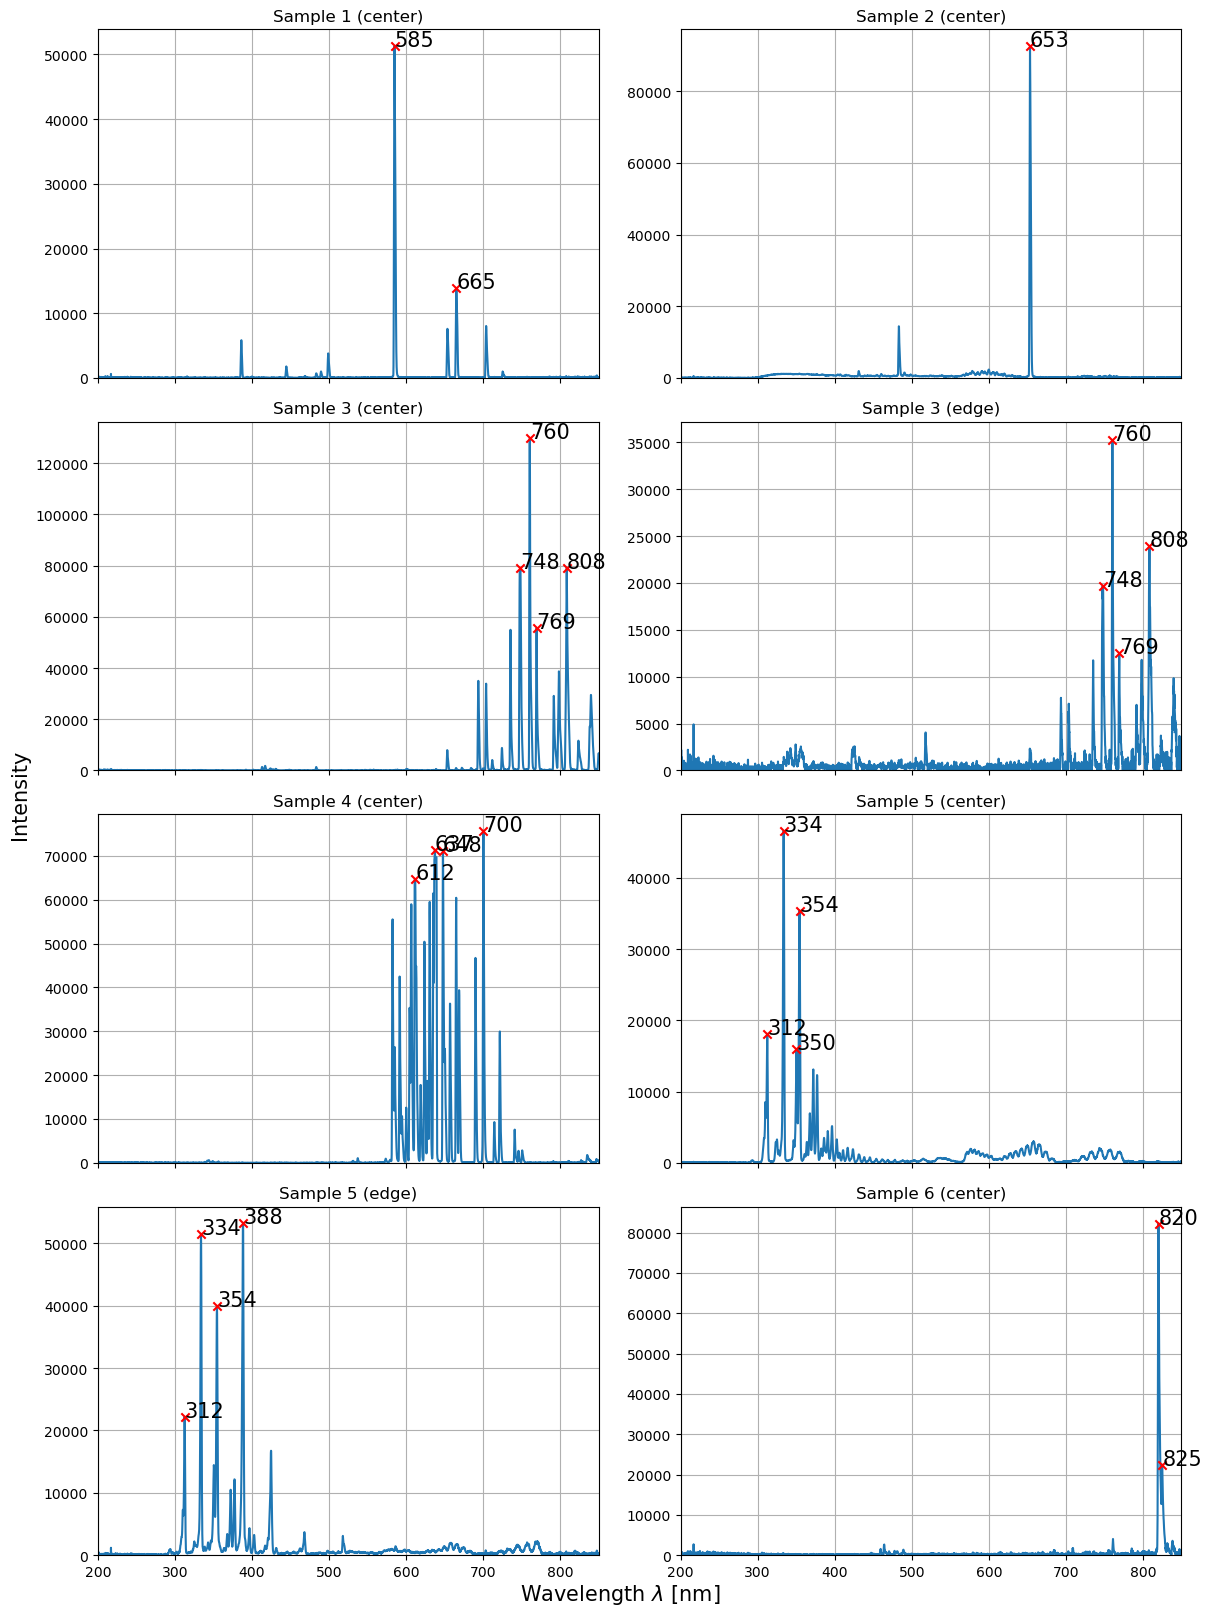
\includegraphics[width=0.98\columnwidth]{./images/spectrum_samples.png}
    \caption{サンプルのスペクトルの測定結果}
    \label{fig:spectrum_samples}
\end{figure}
図\ref{fig:spectrum_samples}に、サンプルのスペクトルの測定結果を示す。
サンプル1はピークが$\SI{585}{nm}, \SI{665}{nm}$であり、ヘリウムランプと推測される。
サンプル2はピークが$\SI{653}{nm}, \SI{480}{nm}$であり、水素ランプと推測される。
サンプル3はピークが$\SI{760}{nm}, \SI{748}{nm}, \SI{808}{nm}$であり、アルゴンランプと推測される。
サンプル4はピークが$\SI{700}{nm}, \SI{648}{nm}, \SI{637}{nm}$等であり、ネオンランプと推測される。
サンプル5はピークが$\SI{388}{nm}, \SI{334}{nm}, \SI{354}{nm}$であり、窒素ランプと推測される。
サンプル6はピークが$\SI{820}{nm}, \SI{825}{nm}$であり、キセノンランプと推測される。

\subsection{ディスプレイの観測}
\begin{figure}
    \centering
    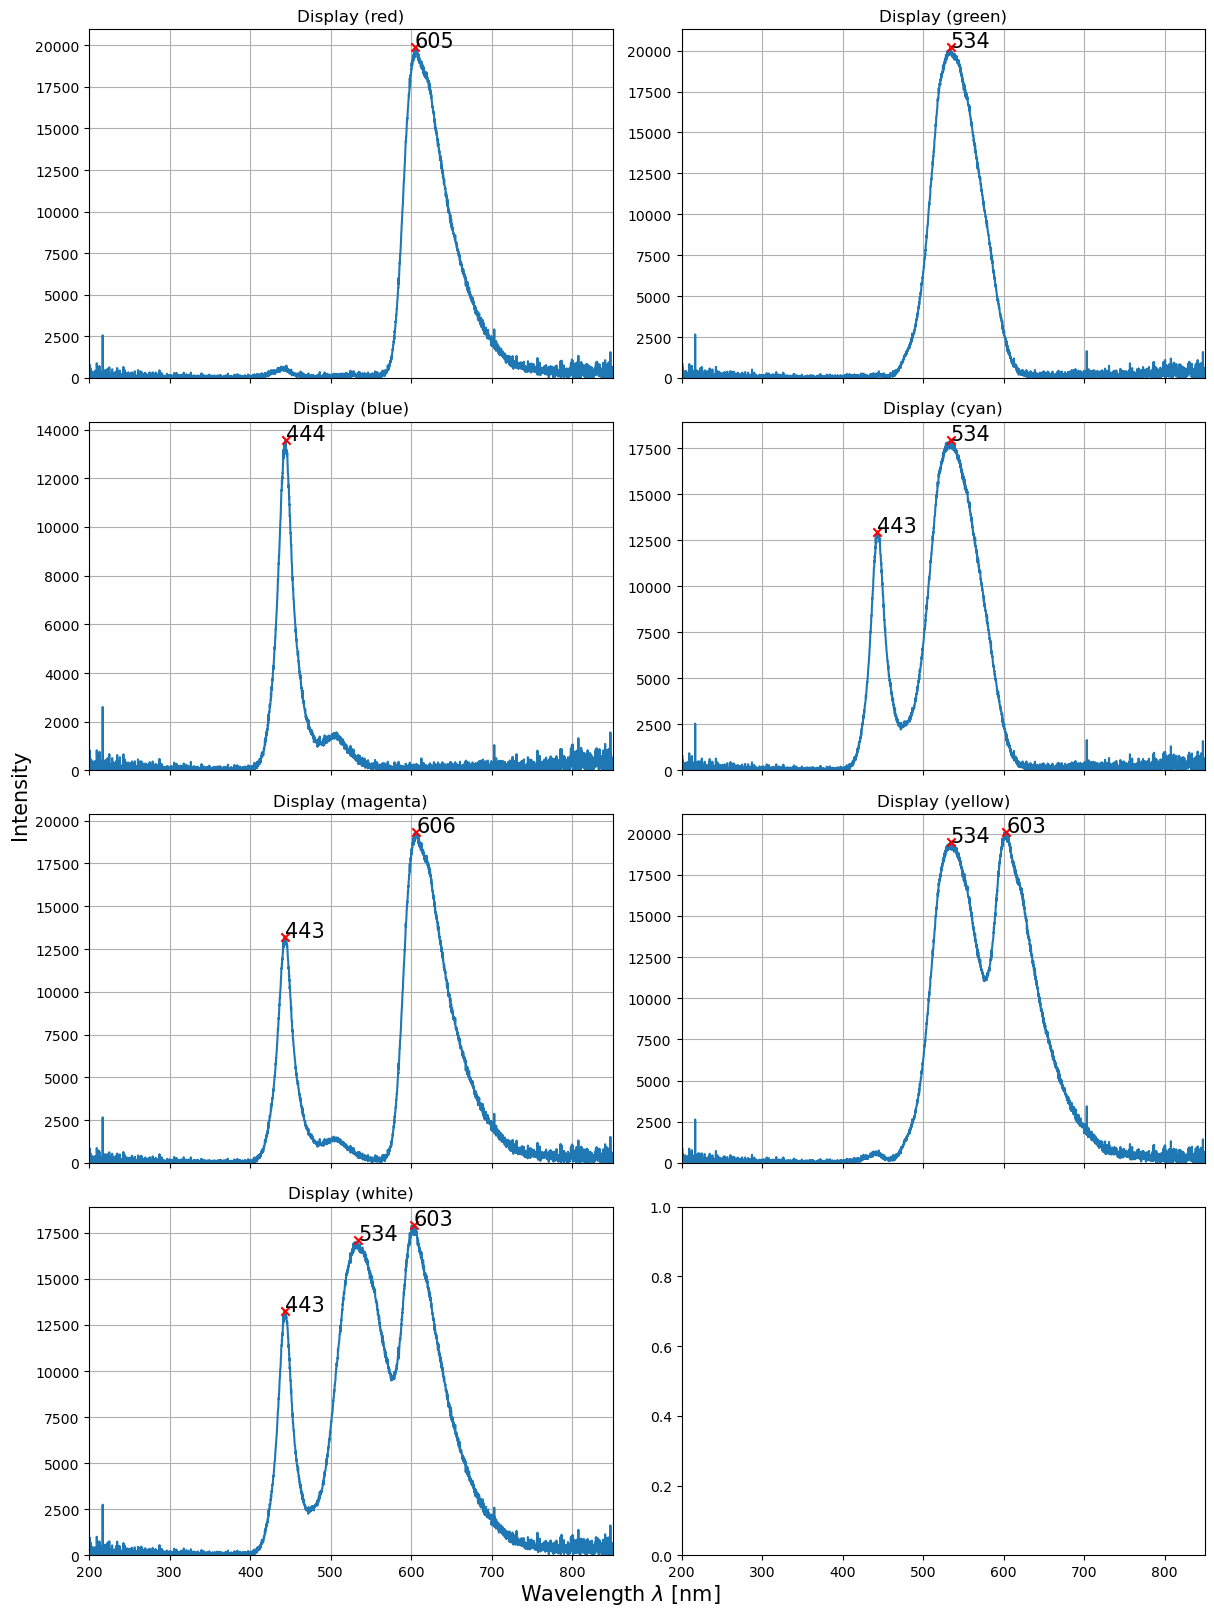
\includegraphics[width=0.98\columnwidth]{./images/spectrum_displays.png}
    \caption{ディスプレイのスペクトルの測定結果}
    \label{fig:spectrum_display}
\end{figure}
図\ref{fig:spectrum_display}に、ディスプレイのスペクトルの測定結果を示す。
光の三原色と言われているRGBはそれぞれ、$\SI{603}{nm}, \SI{534}{nm}, \SI{443}{nm}$であった。
また、CMYおよびWはそれぞれ、RGBの色の合成であることがわかる。

\subsection{その他の観測}
\begin{figure}
    \centering
    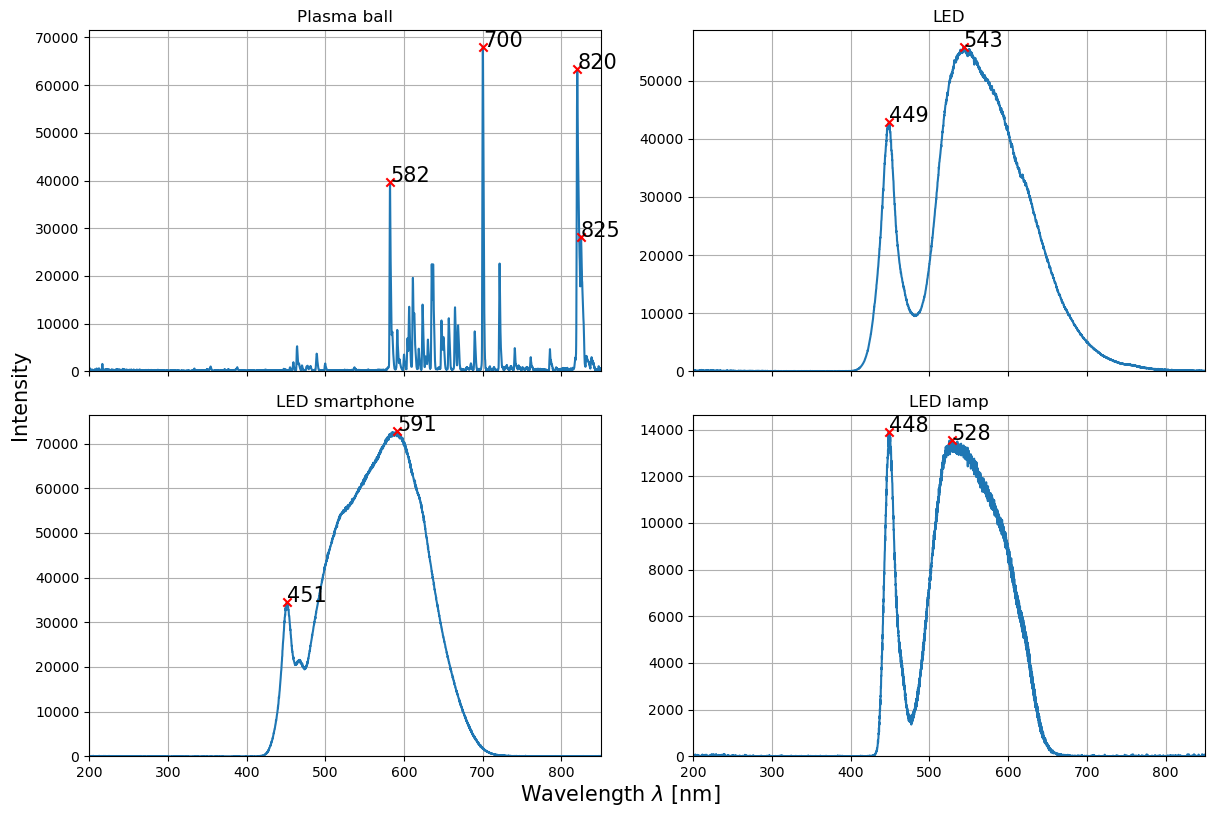
\includegraphics[width=0.98\columnwidth]{./images/spectrum_others.png}
    \caption{プラズマボール・LEDのスペクトルの測定結果}
    \label{fig:spectrum_others}
\end{figure}
図\ref{fig:spectrum_others}に、プラズマボール・LEDのスペクトルの測定結果を示す。
プラズマボールはピークが$\SI{700}{nm}, \SI{820}{nm}, \SI{582}{nm}, \SI{825}{nm}$であり、ネオン、キセノン、ヘリウムの3種の希ガスの混合と推測される。

また、LEDについては、いずれも波形に違いはあったが、幅が広い$\SI{550}{nm}$と鋭い$\SI{450}{nm}$の2箇所のピークがいずれのLEDにも見られた。
これは、白色LEDの発光原理である青色LEDによる蛍光体の励起によるものと考えられる\cite{Webpage 1}。
鋭い$\SI{450}{nm}$のピークは青色LEDの発光によるものであり、広い$\SI{550}{nm}$のピークは蛍光体の発光によるものである。

\subsection{Gaussianによるスペクトル同定}
水素の系列は$n^2$に縮退していることを考慮し、Balmer系列のスペクトルを求めた。
その結果、$H_\alpha = \SI{656}{nm}$、$H_\beta = \SI{486}{nm}$、$H_\gamma = \SI{434}{nm}$、$H_\delta = \SI{410}{nm}$となった。
これは、教科書に記述されていた実際の水素のスペクトル$\SI{656}{nm}$、$\SI{486}{nm}$と一致した。

ただし、シミュレーションを走らせているときに気づいたのだが、Gaussianというソフトウェアは異なるハードウェアで走らせると結果が異なることがある。
そのため、あまりシミュレーション自体の結果が正確でない可能性が存在する。

次に、Heの同定だが、電子のスピンが変わることはないという制約上、取りうる値を計算した。
しかし、先ほど述べたようにハードウェア間での誤差が非常に大きく、また、縮退の順番が入れ替わる(p軌道より先にd軌道が現れる、など)ことも多々あった。
そのため、誤差も$\SI{10}{nm}$程度は存在するが、$\SI{388}{nm}$は$2^3S-3^3P$の遷移、$\SI{447}{nm}$は$2^3S-4^3P$の遷移、$\SI{502}{nm}$は$2^1P-4^1S$の遷移、
$\SI{588}{nm}$は$2^3P-3^3D$の遷移、$\SI{668}{nm}$は$2^1P-3^1D$の遷移、$\SI{706}{nm}$は$2^3P-3^3S$の遷移であると推測される。

\subsection{窒素の振動温度}
\begin{figure}[htbp]
    \centering
    \begin{minipage}[c]{0.48\columnwidth}
        \centering
        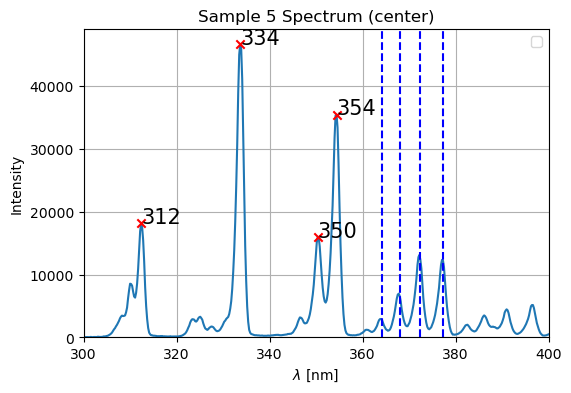
\includegraphics[width=0.95\columnwidth]{./images/spectrum_N2_center.png}
        \subcaption{中央付近のスペクトル}
    \end{minipage}
    \begin{minipage}[c]{0.48\columnwidth}
        \centering
        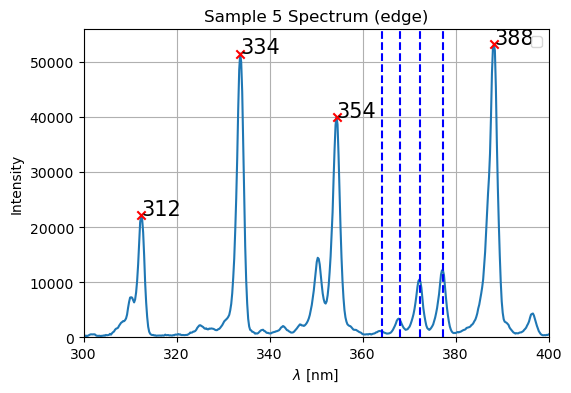
\includegraphics[width=0.95\columnwidth]{./images/spectrum_N2_edge.png}
        \subcaption{端付近のスペクトル}
    \end{minipage}
    \caption{窒素(サンプル5)のスペクトルの測定結果}
    \label{fig:spectrum_nitrogen}
\end{figure}
図\ref{fig:spectrum_nitrogen}は窒素(サンプル5)の$300\sim400\si{nm}$付近のスペクトルを示す。
図の青い点線は、SP02系列の、SP02, SP13, SP24, SP35であり、それぞれ$380,  375, 371, 367\,\si{nm}$である(ただし、それぞれピークと重なるように$\SI{3}{nm}$程ずらしている)。
これらのピークの位置を用いて、振動温度を求めることができる。
\begin{figure}[htbp]
    \centering
    \begin{minipage}[c]{0.48\columnwidth}
        \centering
        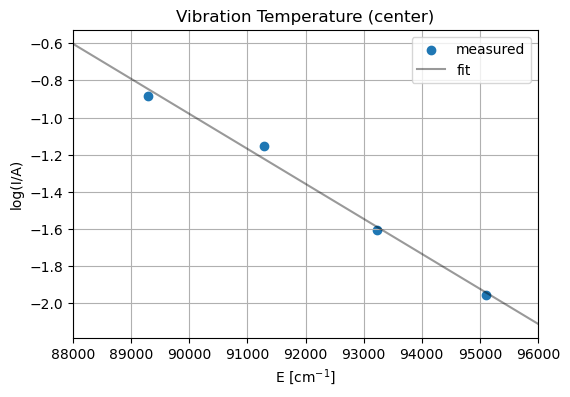
\includegraphics[width=0.95\columnwidth]{./images/spectrum_N2_center_plot.png}
        \subcaption{中央付近の振動温度}
    \end{minipage}
    \begin{minipage}[c]{0.48\columnwidth}
        \centering
        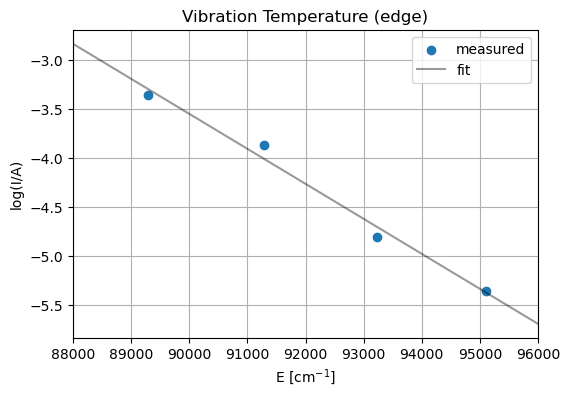
\includegraphics[width=0.95\columnwidth]{./images/spectrum_N2_edge_plot.png}
        \subcaption{端付近の振動温度}
    \end{minipage}
    \caption{窒素(サンプル5)のスペクトルの測定結果}
    \label{fig:spectrum_nitrogen}
\end{figure}
この結果、中央付近での温度は$\SI{7600}{\degreeCelsius}$、端付近での温度は$\SI{4000}{\degreeCelsius}$であった。

\begin{thebibliography}{99}
    \bibitem{Report 1} Berzak, L. F., Dorfman, S. E., \& Smith, S. P. (2006). Paschen’s Law in Air and Noble Gases. \url{https://www-eng.lbl.gov/~shuman/XENON/REFERENCES&OTHER_MISC/paschen_report.pdf}
    \bibitem{Report 2} Massarczyk, R., Chu, P., Dugger, C., Elliott, S., Rielage, K., \& Xu, W. (2017). Paschen’s law studies in cold gases. Journal of Instrumentation, 12(06), P06019. \url{https://doi.org/10.1088/1748-0221/12/06/p06019}
    \bibitem{Journal 1} Radwan, S. I., El-Khabeary, H., \& Helal, A. (2016). Study of the secondary electron emission coefficient using disc and conical electrodes. Canadian Journal of Physics, 94(12), 1275–1281. \url{https://doi.org/10.1139/cjp-2016-0334}
    \bibitem{Webpage 1} 白色LEDのスペクトル. (2012, February 16). 光と色と. Retrieved June 25, 2024, from \url{https://optica.cocolog-nifty.com/blog/2012/02/led-d2e3.html}
    \bibitem{Journal 2} Isa, H. (1971). 球対球, 棒対平板電極の電界計算とその絶縁破壊電圧の計算への応用. 電氣學會雜誌, 91(9). \url{https://doi.org/10.11526/ieejjournal1888.91.9_1730}
    \bibitem{Journal 3} Isa, H. (1980). 雷インパルス電圧による大気圧空気の絶縁破壊現象の観察. Kyoto University. \url{https://doi.org/10.14989/doctor.r4053}
\end{thebibliography}

\end{document}